%==============================================================
%  EE201 -- Circuit Theory I
%  Lecture 11 : Node Voltage Analysis
%  M. Mert Ankaralı, METU EEE
%
%  Compile:  ./build.sh      (or: pdflatex EE201_Lecture_11.tex, twice)
%==============================================================
\documentclass[11pt,a4paper]{article}

%-------------------- packages --------------------------------
\usepackage[T1]{fontenc}
\usepackage[utf8]{inputenc}
\usepackage[english]{babel}
\usepackage{lmodern}
\usepackage[margin=2.3cm,top=2.0cm,bottom=1.9cm,headheight=14pt,headsep=9pt]{geometry}
\usepackage{amsmath,amssymb}
\usepackage{array,booktabs,tabularx}
\usepackage{enumitem}
\usepackage{needspace}
\usepackage[table]{xcolor}
\usepackage{fancyhdr}
\usepackage{titlesec}
\usepackage{graphicx}
\usepackage[most]{tcolorbox}
\usepackage{tikz}
\usepackage[american,siunitx]{circuitikz}
\usetikzlibrary{matrix,arrows.meta,positioning,calc,decorations.pathmorphing,decorations.pathreplacing,decorations.markings,patterns,shapes.geometric}
\usepackage[colorlinks=true,allcolors=metured,breaklinks=true]{hyperref}

%-------------------- colour system ---------------------------
% One colour per physical quantity, used identically in the slides.
\definecolor{metured}{RGB}{155,27,48}    % headings, structure
\definecolor{metugray}{RGB}{88,89,91}
\definecolor{ccur}{RGB}{0,102,170}       % CURRENT  -- blue
\definecolor{cvolt}{RGB}{214,120,0}      % VOLTAGE  -- orange
\definecolor{cpow}{RGB}{23,128,74}       % POWER / ENERGY -- green
\definecolor{ccharge}{RGB}{124,60,160}   % CHARGE   -- purple
\definecolor{cflux}{RGB}{0,138,138}      % FLUX -- teal
\definecolor{boxgray}{RGB}{245,245,245}
\definecolor{copper}{RGB}{184,98,30}

\newcommand{\Icol}[1]{\textcolor{ccur}{#1}}
\newcommand{\Vcol}[1]{\textcolor{cvolt}{#1}}
\newcommand{\Pcol}[1]{\textcolor{cpow}{#1}}
\newcommand{\Qcol}[1]{\textcolor{ccharge}{#1}}
\newcommand{\Fcol}[1]{\textcolor{cflux}{#1}}

%-------------------- units (no siunitx dependency) -----------
\newcommand{\uni}[1]{\,\mathrm{#1}}
\newcommand{\A}{\uni{A}}   \newcommand{\V}{\uni{V}}
\newcommand{\W}{\uni{W}}   \newcommand{\J}{\uni{J}}
\newcommand{\Cb}{\uni{C}}  \newcommand{\s}{\uni{s}}
\newcommand{\Sie}{\uni{S}} \newcommand{\Wb}{\uni{Wb}}

%-------------------- layout ----------------------------------
\pagestyle{fancy}
\fancyhf{}
\lhead{\small\textcolor{metugray}{EE201 -- Circuit Theory I}}
\rhead{\small\textcolor{metugray}{Lecture 11: Node Voltage Analysis}}
\cfoot{\small\thepage}
\renewcommand{\headrulewidth}{0.4pt}

\titleformat{\section}{\large\bfseries\color{metured}}{\thesection.}{0.6em}{}
\titleformat{\subsection}{\normalsize\bfseries\color{metugray}}{\thesubsection.}{0.6em}{}
\titlespacing*{\section}{0pt}{1.4ex plus .3ex}{0.7ex}
\titlespacing*{\subsection}{0pt}{1.1ex plus .2ex}{0.5ex}

\setlist[itemize]{itemsep=2pt,topsep=3pt,parsep=0pt,leftmargin=1.5em}
\setlist[enumerate]{itemsep=2pt,topsep=3pt,parsep=0pt,leftmargin=1.7em}
\setlength{\parindent}{0pt}
\setlength{\parskip}{0.7ex plus .1ex}
\raggedbottom
\widowpenalty=10000
\clubpenalty=10000
\brokenpenalty=10000

%-------------------- boxes -----------------------------------
\newtcolorbox{definitionbox}[1]{enhanced,
  colback=metured!4, colframe=metured, boxrule=0.9pt,
  fonttitle=\bfseries, title={#1}, arc=2pt,
  left=7pt,right=7pt,top=5pt,bottom=5pt, before skip=7pt, after skip=7pt,
  before upper={\setlength{\parskip}{0.6ex plus .1ex}}}

\newtcolorbox{ideabox}[1][Key idea]{enhanced,
  colback=ccur!5, colframe=ccur, boxrule=0.9pt,
  fonttitle=\bfseries, title={#1}, arc=2pt,
  left=7pt,right=7pt,top=5pt,bottom=5pt, before skip=7pt, after skip=7pt,
  before upper={\setlength{\parskip}{0.6ex plus .1ex}}}

\newtcolorbox{examplebox}[1][Example]{enhanced,
  colback=cpow!4, colframe=cpow, boxrule=0.9pt,
  fonttitle=\bfseries, title={#1}, arc=2pt,
  left=7pt,right=7pt,top=5pt,bottom=5pt, before skip=7pt, after skip=7pt,
  before upper={\setlength{\parskip}{0.6ex plus .1ex}}}

\newtcolorbox{cautionbox}[1][Careful]{enhanced,
  colback=cvolt!6, colframe=cvolt, boxrule=0.9pt,
  fonttitle=\bfseries, title={#1}, arc=2pt,
  left=7pt,right=7pt,top=5pt,bottom=5pt, before skip=7pt, after skip=7pt,
  before upper={\setlength{\parskip}{0.6ex plus .1ex}}}

%-------------------- circuitikz defaults ---------------------
%  voltage sources: smaller + and - inside the circle, further apart
\ctikzset{bipoles/vsourceam/inner plus={\tiny$+$},
          bipoles/vsourceam/inner minus={\tiny$\vphantom{+}-$},
          bipoles/vsourceam/margin=0.85,
          bipoles/cvsourceam/inner plus={\tiny$+$},
          bipoles/cvsourceam/inner minus={\tiny$\vphantom{+}-$},
          bipoles/cvsourceam/margin=0.85}
\ctikzset{bipoles/length=0.9cm, color=black,
          label/align=straight,
          bipoles/generic/height=0.28, bipoles/generic/width=0.62}
\tikzset{
  iar/.style={-{Stealth[length=2.2mm]}, ccur, thick},
  pol/.style={font=\small, text=cvolt},
  glab/.style={font=\footnotesize, text=metured},
  ttl/.style={font=\scriptsize\bfseries, text=metugray},
  capn/.style={font=\scriptsize, text=metugray, align=center},
  bigarr/.style={-{Stealth[length=3mm]}, very thick, metugray},
  gnode/.style={circle, fill=metured, inner sep=0pt, minimum size=4.4pt},
  nlab/.style={circle, draw=metured, text=metured, font=\scriptsize, inner sep=0.7pt},
  blab/.style={font=\footnotesize, text=black!80},
  gbr/.style={black!75, thick, postaction={decorate, decoration={markings,
      mark=at position 0.56 with {\arrow{Stealth[length=2.5mm]}}}}},
  apbr/.style={ccur, line width=1.7pt, postaction={decorate, decoration={markings,
      mark=at position 0.56 with {\arrow{Stealth[length=2.8mm]}}}}},
  hal/.style={draw=cpow!60, line width=6pt, opacity=0.35, line cap=round, line join=round},
  elem/.style={draw=metugray, thick, fill=metulight},
}
\definecolor{metulight}{RGB}{243,240,241}

%-------------------- Lecture 11 circuit macros ---------------
\newcommand{\ohm}{\,\Omega}
%  Colour-coded matrix entries: diagonal, off-diagonal, right side (#1 = colour of the right side)
\newcommand{\cbx}[2]{{\setlength{\fboxsep}{1.6pt}\colorbox{#1}{$\displaystyle #2\mathstrut$}}}
\newcommand{\dg}[1]{\cbx{cpow!16}{#1}}
\newcommand{\od}[1]{\cbx{metured!13}{#1}}
\newcommand{\chip}[1]{\textcolor{#1}{$\blacksquare$}}

%  A highlighted matrix row entry: colour #1, content #2
\newcommand{\hrow}[2]{{\setlength{\fboxsep}{1.5pt}\colorbox{#1}{\makebox[2.1em]{$\mathstrut #2$}}}}
\newcommand{\e}[1]{\textcolor{cvolt}{e_{#1}}}
\newcommand{\ep}[1]{\textcolor{cvolt}{e_{#1}'}}
\newcommand{\nd}[1]{\tikz[baseline=(c.base)]\node[nlab](c){#1};}
\newcommand{\vbf}[1]{\textcolor{cvolt}{\mathbf{#1}}}
\newcommand{\ibf}[1]{\textcolor{ccur}{\mathbf{#1}}}
%  A node: dot at (#1) with label #3 placed at anchor #2
\newcommand{\nodev}[3]{\fill (#1) circle (1.7pt) node[#2, inner sep=2pt, font=\small, text=cvolt] {#3};}
%  Ground symbol below (#1,0)
\newcommand{\gnd}[1]{\draw (#1,0) -- (#1,-0.2) node[ground] {};}
%  Examples 11.1 and 11.2.
%  #1 = 0: i_s1, R1..R5 (R5 from node 1 to node 3), i_s2 (11.1);  1: i_s, R1..R4, v_s to ground (11.2);
%  2: as 1, e_3 not a label (11.2 revisited)
%  Stage of Example 11.1 drawings: 0 bare, 1 with the ground, 2 also node voltages (default)
\newcount\exAst \exAst=2
\newcommand{\nodeA}[3]{\ifnum\exAst>1 \nodev{#1}{#2}{#3}\else\fill (#1) circle (1.7pt);\fi}
\newcommand{\exA}[1]{%
  \ifnum#1=0
    \draw (0,0) to[american current source, l=$\Icol{i_{s1}}$] (0,2);
  \else
    \draw (0,0) to[american current source, l=$\Icol{i_s}$] (0,2);
  \fi
  \draw (0,2) -- (1.8,2) to[R, l=$R_2$] (3.8,2) to[R, l_=$R_4$] (5.8,2);
  \draw (1.8,2) to[R, l_=$R_1$] (1.8,0);
  \draw (3.8,2) to[R, l_=$R_3$] (3.8,0);
  \draw (0,0) -- (5.8,0);
  \ifnum#1=0
    \draw (1.8,2) -- (1.8,3.0) to[R, l=$R_5$] (5.8,3.0) -- (5.8,2);
    \draw (5.8,2) to[american current source, l=$\Icol{i_{s2}}$] (5.8,0);
    \nodeA{3.8,2}{above}{$e_2$}
    \nodeA{5.8,2}{above right}{$e_3$}
    \nodeA{1.8,2}{above left}{$e_1$}
  \else
    \draw (5.8,0) to[american voltage source, invert, l_=$\Vcol{v_s}$] (5.8,2);
    \nodev{3.8,2}{above}{$e_2$}
    \ifnum#1=1 \nodev{5.8,2}{above}{$e_3$}\else \fill (5.8,2) circle (1.7pt);\fi
  \fi
  \ifnum#1=0\else\nodeA{1.8,2}{above}{$e_1$}\fi
  \ifnum\exAst>0 \gnd{3.8}\fi}
%  Example 11.3: two voltage sources; v_s2 between nodes 1 and 2.
%  #1 = 0: plain;  1: current i through v_s2;  2: the supernode
\newcommand{\exB}[1]{%
  \draw (0,0) to[american voltage source, invert, l=$\Vcol{v_{s1}}$] (0,2);
  \draw (0,2) to[R, l=$R_1$] (1.8,2) to[american voltage source, l=$\Vcol{v_{s2}}$] (3.6,2)
        to[R, l=$R_4$] (5.4,2) -- (7.0,2);
  \draw (1.8,2) to[R, l=$R_2$] (1.8,0);
  \draw (3.6,2) to[R, l=$R_3$] (3.6,0);
  \draw (5.4,0) to[american current source, l_=$\Icol{i_{s1}}$] (5.4,2);
  \draw (7.0,2) to[R, l=$R_5$] (7.0,0);
  \draw (0,0) -- (7.0,0);
  \nodev{1.8,2}{above right}{$e_1$}
  \nodev{3.6,2}{above left}{$e_2$}
  \nodev{5.4,2}{above}{$e_3$}
  \ifnum#1=1
    \draw[iar] (2.55,1.5) -- (3.05,1.5);
    \node[font=\small, text=ccur] at (2.8,1.25) {$i$};
  \fi
  \ifnum#1=2
    \draw[dashed, metured, thick, rounded corners=4pt] (1.5,1.6) rectangle (3.9,2.95);
    \node[font=\scriptsize, text=metured, anchor=south] at (2.7,2.95) {supernode};
  \fi
  \gnd{1.8}}
%  Example 11.4: a dependent voltage source v_x between nodes 3 and 2.
%  #1 = 0: plain;  1: the supernode S;  2: node 3 as the ground (e1', e2', e4');
%  3: node numbers, ground at the bottom;  4: node numbers, node 3 as the ground
\newcommand{\exC}[1]{%
  \draw (0,0) to[american current source, l=$5\A$] (0,2) -- (0,3.6)
        to[R, l=$2\ohm$] (2.0,3.6)
        to[american controlled voltage source, invert, l=$\Vcol{v_x}$] (5.4,3.6) -- (5.4,2);
  \draw (0,2) -- (2.6,2) to[R, l=$2\ohm$] (5.4,2);
  \draw (2.6,2) to[R, l=$4\ohm$] (2.6,0);
  \draw (5.4,2) to[R, l=$3\ohm$] (5.4,0);
  \draw (0,0) -- (5.4,0);
  \fill (0,2) circle (1.7pt);
  \node[pol] at (2.22,1.55) {$+$}; \node[pol] at (2.22,0.45) {$-$};
  \node[font=\small, text=cvolt] at (1.85,1.0) {$v_x$};
  \ifcase#1
    \nodev{2.6,2}{above left}{$e_1$}\nodev{5.4,2}{above right}{$e_2$}\nodev{2.0,3.6}{above right}{$e_3$}\gnd{2.6}
  \or
    \nodev{2.6,2}{above left}{$e_1$}\nodev{5.4,2}{above right}{$e_2$}\nodev{2.0,3.6}{above right}{$e_3$}\gnd{2.6}
  \or
    \nodev{2.6,2}{above left}{$e_1'$}\nodev{5.4,2}{right}{$e_2'$}
    \fill (2.0,3.6) circle (1.7pt); \draw (2.0,3.6) -- (2.0,3.3) node[ground] {};
    \nodev{2.6,0}{below}{$e_4'$}
  \or
    \fill (2.6,2) circle (1.7pt) node[nlab, above left=1pt] {1};
    \fill (5.4,2) circle (1.7pt) node[nlab, right=2pt] {2};
    \fill (2.0,3.6) circle (1.7pt) node[nlab, above right=1pt] {3};
    \fill (4.0,0) circle (1.7pt) node[nlab, below=2pt] {4};
    \gnd{2.6}
  \or
    \fill (2.6,2) circle (1.7pt) node[nlab, above left=1pt] {1};
    \fill (5.4,2) circle (1.7pt) node[nlab, right=2pt] {2};
    \fill (2.0,3.6) circle (1.7pt) node[nlab, above right=1pt] {3};
    \draw (2.0,3.6) -- (2.0,3.3) node[ground] {};
    \fill (4.0,0) circle (1.7pt) node[nlab, below=2pt] {4};
  \fi
  \ifnum#1=1
    \draw[dashed, metured, thick, rounded corners=4pt]
      (1.7,4.4) -- (6.1,4.4) -- (6.1,1.55) -- (4.95,1.55) -- (4.95,3.05) -- (1.7,3.05) -- cycle;
    \node[nlab] at (6.4,4.4) {S};
  \fi}
%  A first small example: i_s1, R1, R2, R3, i_s2.  #1 = 0: branch voltages and currents only;
%  1: also the ground and the node voltages
\newcommand{\exI}[1]{%
  \draw (0,0) to[american current source, l=$\Icol{i_{s1}}$] (0,2.6) -- (2.4,2.6)
        to[R, l=$R_2$] (5.2,2.6) -- (7.2,2.6);
  \draw (2.4,2.6) to[R, l=$R_1$] (2.4,0);
  \draw (5.2,2.6) to[R, l=$R_3$] (5.2,0);
  \draw (7.2,2.6) to[american current source, l=$\Icol{i_{s2}}$] (7.2,0);
  \draw (0,0) -- (7.2,0);
  \node[pol] at (2.05,1.75) {$+$}; \node[pol] at (2.05,0.85) {$-$};
  \node[font=\small, text=cvolt] at (1.75,1.3) {$v_1$};
  \node[pol] at (3.42,2.25) {$+$}; \node[pol] at (4.25,2.25) {$-$};
  \node[font=\small, text=cvolt] at (3.8,2.22) {$v_2$};
  \node[pol] at (4.85,1.75) {$+$}; \node[pol] at (4.85,0.85) {$-$};
  \node[font=\small, text=cvolt] at (4.55,1.3) {$v_3$};
  \draw[iar] (2.62,2.45) -- (2.62,2.0); \node[font=\small, text=ccur] at (2.88,2.22) {$i_1$};
  \draw[iar] (2.65,2.85) -- (3.1,2.85); \node[font=\small, text=ccur] at (2.88,3.12) {$i_2$};
  \draw[iar] (5.42,2.45) -- (5.42,2.0); \node[font=\small, text=ccur] at (5.68,2.22) {$i_3$};
  \ifnum#1=1
    \nodev{2.4,2.6}{above left}{$e_1$}
    \nodev{5.2,2.6}{above}{$e_2$}
    \gnd{3.8}
  \fi}
%  Example 11.4: a dependent current source 0.5 v_x into node 2, v_x the voltage of the 2 ohm
\newcommand{\exD}{%
  \draw (0,0) to[american current source, l=$1\A$] (0,2) -- (1.6,2) to[R, l=$6\ohm$] (3.6,2) -- (5.2,2);
  \draw (1.6,2) to[R, l=$2\ohm$] (1.6,0);
  \draw (3.6,2) to[R, l=$6\ohm$] (3.6,0);
  \draw (5.2,0) to[american controlled current source, l_=$\Icol{0.5\,v_x}$] (5.2,2);
  \draw (0,0) -- (5.2,0);
  \node[pol] at (1.25,1.55) {$+$}; \node[pol] at (1.25,0.45) {$-$};
  \node[font=\small, text=cvolt] at (0.95,1.0) {$v_x$};
  \nodev{1.6,2}{above}{$e_1$}
  \nodev{3.6,2}{above}{$e_2$}
  \gnd{2.6}}
%  Graph branch from #1 to #2, label #4 on side #3 (angle), optional colour #5
\newcommand{\gbranch}[5][black!75]{%
  \draw[gbr, #1] (#2) -- (#3);
  \node[blab, text=#1] at ($(#2)!0.5!(#3)!0.3cm!#4:(#3)$) {#5};}
%  An incidence matrix with node labels on the left and branch numbers on top.
%  #1 name, #2 number of columns, #3 node labels, #4 rows (entries separated by \&), #5 extra TikZ
\newcommand{\incmat}[5]{%
  \begin{tikzpicture}[baseline={([yshift=-0.6ex]#1.center)}]
    \matrix (#1) [matrix of math nodes, ampersand replacement=\&,
                  left delimiter={[}, right delimiter={]}, inner sep=1pt,
                  column sep=0.45em,
                  nodes={text width=1.35em, align=right, minimum height=1.25em,
                         inner sep=1pt}] {#4};
    \foreach \j in {1,...,#2}
      \node[font=\scriptsize, text=metugray, anchor=south east, inner sep=1pt]
        at ([yshift=2pt]#1-1-\j.north east) {\j};
    \foreach \lab [count=\i] in {#3}
      \node[nlab, left=11pt] at (#1.west |- #1-\i-1) {\lab};
    #5
  \end{tikzpicture}}
%  The graph of Example 11.1: branches 1-5 the resistors R1-R5, 6 and 7 the sources i_s1, i_s2;
%  node 0 is the ground
\newcommand{\exAgraph}{%
  \coordinate (g1) at (0,1.6); \coordinate (g2) at (2.2,1.6);
  \coordinate (g3) at (4.4,1.6); \coordinate (g0) at (2.2,0);
  \gbranch{g1}{g0}{90}{1}
  \gbranch{g1}{g2}{90}{2}
  \gbranch{g2}{g0}{90}{3}
  \gbranch{g2}{g3}{90}{4}
  \draw[gbr] (g1) to[bend left=45] (g3); \node[blab] at (2.2,2.75) {5};
  \draw[gbr, ccur] (g0) to[bend left=50] (g1); \node[blab, text=ccur] at (0.45,0.25) {6};
  \gbranch[ccur]{g3}{g0}{-90}{7}
  \foreach \k/\pos in {1/left, 2/above, 3/right, 0/below}
    {\fill[metured] (g\k) circle (2.2pt); \node[nlab, \pos=3pt] at (g\k) {\k};}}
%  The reduced incidence matrix of Example 11.1 (rows: nodes 1, 2, 3)
%  \exAincN{k}: the reduced A of Example 11.1 with its first k rows filled in; k = 4 adds the
%  A_R / A_S boxes
\newcommand{\exAincN}[1]{%
  \ifnum#1>0 \def\rowA{1 \& 1 \& 0 \& 0 \& 1 \& \textcolor{ccur}{-1} \& \textcolor{ccur}{0}}%
  \else\def\rowA{\phantom{0} \& \phantom{0} \& \phantom{0} \& \phantom{0} \& \phantom{0} \& \phantom{0} \& \phantom{0}}\fi
  \ifnum#1>1 \def\rowB{0 \& -1 \& 1 \& 1 \& 0 \& \textcolor{ccur}{0} \& \textcolor{ccur}{0}}%
  \else\def\rowB{\phantom{0} \& \phantom{0} \& \phantom{0} \& \phantom{0} \& \phantom{0} \& \phantom{0} \& \phantom{0}}\fi
  \ifnum#1>2 \def\rowC{0 \& 0 \& 0 \& -1 \& -1 \& \textcolor{ccur}{0} \& \textcolor{ccur}{1}}%
  \else\def\rowC{\phantom{0} \& \phantom{0} \& \phantom{0} \& \phantom{0} \& \phantom{0} \& \phantom{0} \& \phantom{0}}\fi
  \incmat{AA}{7}{1,2,3}{\rowA\\ \rowB\\ \rowC\\}{%
    \ifnum#1>3
    \draw[metugray, thick, rounded corners=2pt]
      ([xshift=-2pt, yshift=1pt]AA-1-1.north west) rectangle ([xshift=2pt, yshift=-1pt]AA-3-5.south east);
    \draw[ccur, thick, rounded corners=2pt]
      ([xshift=-2pt, yshift=1pt]AA-1-6.north west) rectangle ([xshift=2pt, yshift=-1pt]AA-3-7.south east);
    \node[font=\small, text=metugray, below=3pt] at ($(AA-3-1.south)!0.5!(AA-3-5.south)$) {$A_R$: resistors};
    \node[font=\small, text=ccur, below=3pt] at ($(AA-3-6.south)!0.5!(AA-3-7.south)$) {$A_S$: sources};
    \else
    \node[font=\small, below=3pt] at ($(AA-3-1.south)!0.5!(AA-3-5.south)$) {\phantom{$A_R$: resistors}};
    \fi}}
\newcommand{\exAinc}{\exAincN{4}}
%  Example 11.6: one circuit, two grounds.  #1 = ground node (3: bottom, 2: top right);
%  #2 = 0: node numbers; 1: node voltages
\newcommand{\exG}[2]{%
  \path (-1.2,-0.8) rectangle (6.1,2.45);
  \draw (0,0) to[american current source, l=$7\A$] (0,1.8) -- (2.2,1.8)
        to[R, l=$2\ohm$] (5.0,1.8);
  \draw (2.2,1.8) to[R, l_=$1\ohm$] (2.2,0);
  \draw (5.0,1.8) to[R, l_=$4\ohm$] (5.0,0);
  \draw (0,0) -- (5.0,0);
  \ifnum#1=3 \gnd{3.6}\else \draw (5.0,1.8) -- (5.7,1.8) -- (5.7,1.6) node[ground] {};\fi
  \ifnum#2=0
    \fill (2.2,1.8) circle (1.7pt) node[nlab, above left=1pt] {1};
    \fill (5.0,1.8) circle (1.7pt) node[nlab, above=2pt] {2};
    \fill (3.6,0) circle (1.7pt) node[nlab, below right=1pt] {3};
  \else\ifnum#1=3
    \nodev{2.2,1.8}{above left}{$e_1$}\nodev{5.0,1.8}{above}{$e_2$}
  \else
    \nodev{2.2,1.8}{above left}{$e_1'$}\fill (5.0,1.8) circle (1.7pt);
    \nodev{3.6,0}{below}{$e_3'$}
  \fi\fi}
\tikzset{fbox/.style={draw=metugray, thick, fill=metulight, rounded corners=3pt,
                      minimum height=0.85cm, minimum width=1.4cm, align=center,
                      font=\small, inner sep=4pt}}

\begin{document}

%-------------------- title block -----------------------------
\begin{center}
\begin{tcolorbox}[enhanced, colback=metured!5, colframe=metured, boxrule=1pt,
                  arc=3pt, left=10pt,right=10pt,top=7pt,bottom=7pt, width=\textwidth]
\begin{center}
  {\small\scshape Middle East Technical University}\\[2pt]
  {\small\scshape Department of Electrical and Electronics Engineering}\\[7pt]
  {\Large\bfseries\color{metured} EE201 -- Circuit Theory I}\\[4pt]
  {\large\bfseries Lecture 11: Node Voltage Analysis}\\[6pt]
  {\small M. Mert Ankaralı}
\end{center}
\end{tcolorbox}
\end{center}
\vspace{-0.5em}

\begin{center}
\small
\begin{tabular}{@{}l l@{}}
\toprule
\multicolumn{2}{@{}l}{\textbf{Colour code used in these notes and in the slides}}\\
\midrule
\Icol{$\blacksquare$}~current $i$ \quad \Vcol{$\blacksquare$}~voltage $v$, node voltage $e$ &
\textcolor{metured}{$\blacksquare$}~supernode, nodes \nd{S}\\
\bottomrule
\end{tabular}
\end{center}

\textbf{Motivation.} So far, circuits were solved by simplifying them. Simplifying
fundamentally changes the circuit; that is its whole point. To find the quantities of the
original circuit, we must go back step by step, and some circuits cannot be simplified at all.
\textbf{Node voltage analysis} works on the original circuit, without changing it. It works
for every LTI resistive circuit; voltage sources need small additions, such as the supernode. Its unknowns are only the $n-1$ node voltages; every branch
voltage and current follows from them. Mesh current analysis comes later.

%==============================================================
\section{The procedure, on an example}

For now, the circuit has only resistors and independent current sources; voltage sources and
dependent sources come later. The circuit of Example 11.1 has $b = 7$ branches, so $14$ branch
voltages and currents. Node voltage analysis needs only $3$ unknowns. Four steps find them.

\begin{examplebox}[Example 11.1 --- node voltage analysis step by step]
\begin{minipage}[c]{0.42\linewidth}
\centering
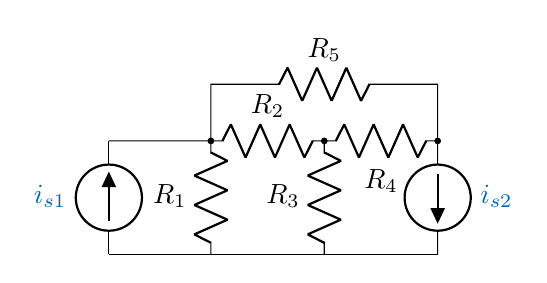
\begin{tikzpicture}[scale=0.72]
  \exA{0}
\end{tikzpicture}
\end{minipage}\hfill
\begin{minipage}[c]{0.56\linewidth}
\begin{enumerate}
  \item \textbf{Reference node.} Choose the bottom node as the ground; its node voltage is $0$.
  \item \textbf{Node voltages.} Label the others $\e{1}$, $\e{2}$, $\e{3}$. Every branch
        voltage is a difference of them ($\Vcol{v_{R_2}} = \e{1} - \e{2}$), so KVL holds automatically.
  \item \textbf{Currents.} The current leaving node $k$ through $R$ to node $j$ is
        $(\e{k} - \e{j})/R$; to the ground, $\e{k}/R$.
  \item \textbf{KCL} at every node except the ground:
\end{enumerate}
\end{minipage}
\begin{alignat*}{2}
  &\text{node 1:}\qquad & -\Icol{i_{s1}} + \frac{\e{1}}{R_1} + \frac{\e{1} - \e{2}}{R_2}
                    + \frac{\e{1} - \e{3}}{R_5} &= 0\\
  &\text{node 2:}\qquad & \frac{\e{2} - \e{1}}{R_2} + \frac{\e{2}}{R_3} + \frac{\e{2} - \e{3}}{R_4} &= 0\\
  &\text{node 3:}\qquad & \frac{\e{3} - \e{2}}{R_4} + \frac{\e{3} - \e{1}}{R_5} + \Icol{i_{s2}} &= 0
\end{alignat*}
The source $\Icol{i_{s1}}$ points into node 1, so it enters with a minus sign. Three equations,
three unknowns; then Steps 2 and 3 give every branch voltage and current.
\end{examplebox}

In general, $\Vcol{\mathbf{v}} = A^T\Vcol{\mathbf{e}}$ (KVL holds automatically), the element
laws give $\Icol{\mathbf{i}}$, and KCL $A\Icol{\mathbf{i}} = \mathbf{0}$ gives $n - 1$ equations
in the $n - 1$ node voltages.

%==============================================================
\section{Matrix form}

With $G_k = 1/R_k$ and the terms collected, the three equations of Example 11.1 become
\[
  \underbrace{\begin{bmatrix}
    \dg{G_1 + G_2 + G_5} & \od{-G_2} & \od{-G_5}\\[2pt]
    \od{-G_2} & \dg{G_2 + G_3 + G_4} & \od{-G_4}\\[2pt]
    \od{-G_5} & \od{-G_4} & \dg{G_4 + G_5}
  \end{bmatrix}}_{Y_n}
  \underbrace{\begin{bmatrix} \e{1}\\[2pt] \e{2}\\[2pt] \e{3} \end{bmatrix}}_{\Vcol{\mathbf{e}}}
  =
  \underbrace{\begin{bmatrix} \cbx{ccur!14}{\Icol{i_{s1}}}\\[2pt] \cbx{ccur!14}{0}\\[2pt] \cbx{ccur!14}{-\Icol{i_{s2}}} \end{bmatrix}}_{\Icol{\mathbf{i}_n}} .
\]
$Y_n$ is the \textbf{node admittance matrix}, and $Y_n\Vcol{\mathbf{e}} = \Icol{\mathbf{i}_n}$
are the \textbf{node equations}; $\Icol{\mathbf{i}_n}$ holds the source currents entering each
node. The three colours follow three rules, so for a circuit of resistors and current sources
the node equations can be written down directly.

\begin{ideabox}[Writing $Y_n$ directly from the circuit: three rules]
\begin{itemize}
  \item \chip{cpow!45} \textbf{Diagonal} entry $(k,k)$: the sum of the conductances connected to node $k$.
  \item \chip{metured!50} \textbf{Off-diagonal} entry $(k,j)$: minus the sum of the conductances between nodes
        $k$ and $j$.
  \item \chip{ccur!45} \textbf{Right side}, row $k$: the sum of the source currents entering node $k$.
\end{itemize}
In Example 11.1:
\par\smallskip
{\centering\small
\renewcommand{\arraystretch}{1.15}
\begin{tabular}{@{}lll@{}}
  \cellcolor{cpow!16}\textbf{Diagonal} & \cellcolor{metured!13}\textbf{Off-diagonal} & \cellcolor{ccur!14}\textbf{Right side}\\
  $(1,1)$: $G_1, G_2, G_5$ meet node 1 & $(1,2)$, $(2,1)$: $G_2$ between 1 and 2 & row 1: $\Icol{i_{s1}}$ enters node 1\\
  $(2,2)$: $G_2, G_3, G_4$ meet node 2 & $(1,3)$, $(3,1)$: $G_5$ between 1 and 3 & row 2: no source\\
  $(3,3)$: $G_4, G_5$ meet node 3 & $(2,3)$, $(3,2)$: $G_4$ between 2 and 3 & row 3: $\Icol{i_{s2}}$ leaves node 3
\end{tabular}\par}
\smallskip
Each conductance between two nodes appears twice, at $(k,j)$ and $(j,k)$: $Y_n$ is
\textbf{symmetric}.
\end{ideabox}

\textbf{$Y_n$ from the graph.} In the graph of Example 11.1, branches 1--5 are the resistors
$R_1, \dots, R_5$, branches 6 and 7 are the sources $\Icol{i_{s1}}$, $\Icol{i_{s2}}$, and node
\nd{0} is the ground. The reduced incidence matrix $A$ has one row for each node except the
ground; an entry is $+1$ if the branch leaves the node and $-1$ if it enters.

\begin{center}
\begin{minipage}[c]{0.4\linewidth}
\centering
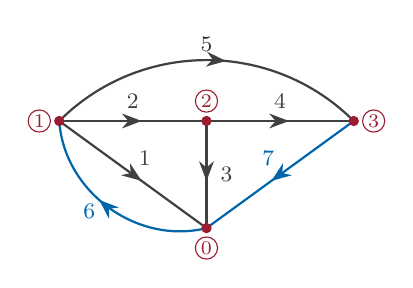
\begin{tikzpicture}[scale=0.85]
  \exAgraph
\end{tikzpicture}
\end{minipage}\hfill
\begin{minipage}[c]{0.56\linewidth}
\centering
$A = \exAinc$
\end{minipage}
\end{center}

KCL $A\Icol{\mathbf{i}} = \mathbf{0}$ reads $A_R\Icol{\mathbf{i}_R} + A_S\Icol{\mathbf{i}_S} = \mathbf{0}$.
The resistors obey $\Icol{\mathbf{i}_R} = G\,\Vcol{\mathbf{v}_R}$ with
$G = \mathrm{diag}(G_1, \dots, G_5)$. KVL, $\Vcol{\mathbf{v}} = A^T\Vcol{\mathbf{e}}$, splits into rows:
$\left[\begin{smallmatrix} \Vcol{\mathbf{v}_R}\\ \Vcol{\mathbf{v}_S} \end{smallmatrix}\right]
= \left[\begin{smallmatrix} A_R^T\\ A_S^T \end{smallmatrix}\right]\Vcol{\mathbf{e}}$, so
$\Vcol{\mathbf{v}_R} = A_R^T\Vcol{\mathbf{e}}$ (resistor rows) and
$\Vcol{\mathbf{v}_S} = A_S^T\Vcol{\mathbf{e}}$ (source rows); only the resistor rows are needed. In
Example 11.1, $A_R^T$ is the resistor columns 1--5 of $A$ written as rows, and
\[
  \Vcol{\mathbf{v}_R} = A_R^T\Vcol{\mathbf{e}}
  = \begin{bmatrix}
    1 & 1 & 0 & 0 & 1\\
    0 & -1 & 1 & 1 & 0\\
    0 & 0 & 0 & -1 & -1
  \end{bmatrix}^T
  \begin{bmatrix} \e{1}\\ \e{2}\\ \e{3} \end{bmatrix}
  = \big[\, \e{1} \ \ \ \e{1} - \e{2} \ \ \ \e{2} \ \ \ \e{2} - \e{3} \ \ \ \e{1} - \e{3} \,\big]^T :
\]
each resistor voltage is its tail node voltage minus its head node voltage. Together,
\[
  A_R\,G\,A_R^T\,\Vcol{\mathbf{e}} = -A_S\Icol{\mathbf{i}_S}
  \quad\Rightarrow\quad
  Y_n = A_R\,G\,A_R^T, \qquad \Icol{\mathbf{i}_n} = -A_S\Icol{\mathbf{i}_S}.
\]
For Example 11.1,
\[
  A_R\,G = \begin{bmatrix}
      G_1 & G_2 & 0 & 0 & G_5\\
      0 & -G_2 & G_3 & G_4 & 0\\
      0 & 0 & 0 & -G_4 & -G_5
    \end{bmatrix},
  \qquad
  -A_S\Icol{\mathbf{i}_S}
    = -\begin{bmatrix} -1 & 0\\ 0 & 0\\ 0 & 1 \end{bmatrix}
       \begin{bmatrix} \Icol{i_{s1}}\\ \Icol{i_{s2}} \end{bmatrix}
    = \begin{bmatrix} \Icol{i_{s1}}\\ 0\\ -\Icol{i_{s2}} \end{bmatrix},
\]
and $A_R\,G\,A_R^T$ is exactly the $Y_n$ above: the three rules read this product off entry by
entry. Finally, $Y_n^T = A_R\,G^T A_R^T = A_R\,G\,A_R^T = Y_n$, since $G$ is diagonal: with
resistors and current sources, $Y_n$ is always symmetric.

%==============================================================
\section{A voltage source to the ground}

\begin{definitionbox}{A voltage source to the ground}
If an independent voltage source $\Vcol{v_s}$ is connected between the ground and node $k$,
then $\e{k} = \Vcol{v_s}$ is known. So $\e{k}$ is not an unknown, and KCL is not written at
node $k$.
\end{definitionbox}

\begin{examplebox}[Example 11.2 --- a voltage source between node 3 and the ground]
\begin{minipage}[c]{0.45\linewidth}
\centering
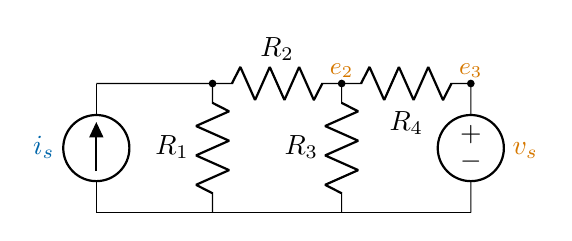
\begin{tikzpicture}[scale=0.82]
  \exA{1}
\end{tikzpicture}
\end{minipage}\hfill
\begin{minipage}[c]{0.52\linewidth}
The source fixes $\e{3} = \Vcol{v_s}$, so the unknowns are only $\e{1}$, $\e{2}$:
\begin{alignat*}{2}
  &\text{node 1:}\quad & -\Icol{i_s} + \frac{\e{1}}{R_1} + \frac{\e{1} - \e{2}}{R_2} &= 0\\
  &\text{node 2:}\quad & \frac{\e{2} - \e{1}}{R_2} + \frac{\e{2}}{R_3} + \frac{\e{2} - \Vcol{v_s}}{R_4} &= 0
\end{alignat*}
\end{minipage}
\end{examplebox}

In matrix form, Example 11.2 reads
\[
  \begin{bmatrix}
    \frac{1}{R_1} + \frac{1}{R_2} & -\frac{1}{R_2}\\[3pt]
    -\frac{1}{R_2} & \frac{1}{R_2} + \frac{1}{R_3} + \frac{1}{R_4}
  \end{bmatrix}
  \begin{bmatrix} \e{1}\\[3pt] \e{2} \end{bmatrix}
  =
  \begin{bmatrix} \Icol{i_s}\\[3pt] \Vcol{v_s}/R_4 \end{bmatrix} .
\]
The known $\Vcol{v_s}$ moves to the right side: $\Vcol{v_s}/R_4$ acts like a current into node 2.

%==============================================================
\section{A voltage source between two nodes: modified node analysis}

If a voltage source (independent or dependent) lies between two nodes and neither is the
ground, KCL there needs its current. Its law fixes its voltage, not its current, so this
current cannot be written with node voltages. \textbf{Modified node analysis} offers two ways out.

\begin{definitionbox}{Method I}
Let the unknown current $\Icol{i}$ through the voltage source be one more unknown. Write KCL at
every node except the ground, and add the law of the source as a \textbf{constraint equation}.
\end{definitionbox}

\begin{examplebox}[Example 11.3 --- Method I]
{\centering
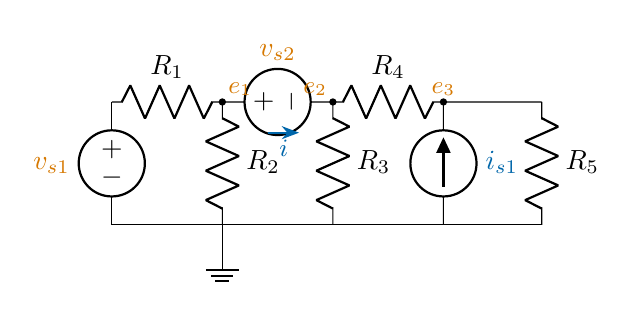
\begin{tikzpicture}[scale=0.78]
  \exB{1}
\end{tikzpicture}\par}
The top of $\Vcol{v_{s1}}$ is at the known voltage $\Vcol{v_{s1}}$; $\Vcol{v_{s2}}$ is between
nodes 1 and 2. Unknowns: $\e{1}$, $\e{2}$, $\e{3}$ and $\Icol{i}$.

\begin{minipage}[c]{0.43\linewidth}
\begin{alignat*}{2}
  &\text{node 1:}\ \ & \frac{\e{1} - \Vcol{v_{s1}}}{R_1} + \frac{\e{1}}{R_2} + \Icol{i} &= 0\\
  &\text{node 2:}\ \ & -\Icol{i} + \frac{\e{2}}{R_3} + \frac{\e{2} - \e{3}}{R_4} &= 0\\
  &\text{node 3:}\ \ & \frac{\e{3} - \e{2}}{R_4} - \Icol{i_{s1}} + \frac{\e{3}}{R_5} &= 0\\
  &\text{constraint:}\ \ & \e{1} - \e{2} &= \Vcol{v_{s2}}
\end{alignat*}
\end{minipage}\hfill
\begin{minipage}[c]{0.55\linewidth}
\small
\[
  \begin{bmatrix}
    G_1 + G_2 & 0 & 0 & 1\\
    0 & G_3 + G_4 & -G_4 & -1\\
    0 & -G_4 & G_4 + G_5 & 0\\
    1 & -1 & 0 & 0
  \end{bmatrix}
  \begin{bmatrix} \e{1}\\ \e{2}\\ \e{3}\\ \Icol{i} \end{bmatrix}
  =
  \begin{bmatrix} G_1\Vcol{v_{s1}}\\ 0\\ \Icol{i_{s1}}\\ \Vcol{v_{s2}} \end{bmatrix}
\]
\end{minipage}

\smallskip
Four unknowns and four equations; the last row is the constraint. This works, but it adds the
unknown $\Icol{i}$; the supernode below avoids it.

\end{examplebox}

\begin{definitionbox}{Method II: the supernode}
Write KCL as if the two nodes of the voltage source were a single node, a
\textbf{supernode}. Add the law of the source as a constraint equation.
\end{definitionbox}

\begin{examplebox}[Example 11.3, revisited --- Method II, three unknowns]
\begin{minipage}[c]{0.44\linewidth}
\centering
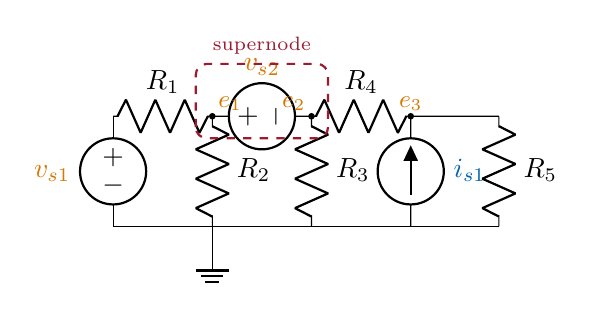
\begin{tikzpicture}[scale=0.7]
  \exB{2}
\end{tikzpicture}
\end{minipage}\hfill
\begin{minipage}[c]{0.54\linewidth}
\small
\begin{alignat*}{2}
  &\text{supernode:}\ \ & \frac{\e{1} - \Vcol{v_{s1}}}{R_1} + \frac{\e{1}}{R_2} + \frac{\e{2}}{R_3}
                       + \frac{\e{2} - \e{3}}{R_4} &= 0\\
  &\text{node 3:}\ \ & \frac{\e{3} - \e{2}}{R_4} - \Icol{i_{s1}} + \frac{\e{3}}{R_5} &= 0\\
  &\text{constraint:}\ \ & \e{1} - \e{2} &= \Vcol{v_{s2}}
\end{alignat*}
\end{minipage}
\end{examplebox}

\textbf{Why does it work?} Add the KCL equations of nodes 1 and 2 in Method I: $\Icol{i}$
leaves node 1 and enters node 2, so it cancels. The sum is KCL around the supernode.
The current $\Icol{i}$ is no longer needed. In matrix form, with three unknowns and three equations:
\[
  \begin{bmatrix}
    G_1 + G_2 & G_3 + G_4 & -G_4\\
    0 & -G_4 & G_4 + G_5\\
    1 & -1 & 0
  \end{bmatrix}
  \begin{bmatrix} \e{1}\\ \e{2}\\ \e{3} \end{bmatrix}
  =
  \begin{bmatrix} G_1\Vcol{v_{s1}}\\ \Icol{i_{s1}}\\ \Vcol{v_{s2}} \end{bmatrix} .
\]
The matrix is no longer symmetric.

Method II needs one unknown fewer than Method I and gives the same node voltages; the current
$\Icol{i}$, if needed, follows from a KCL afterwards.

%==============================================================
\section{Dependent sources}

A dependent source is treated like an independent source of the same kind. Its control
variable is written with node voltages. First plug this into the equations, then form the
matrix. A dependent source makes $Y_n$ not symmetric.

\begin{examplebox}[Example 11.4 --- a dependent current source]
\begin{minipage}[c]{0.42\linewidth}
\centering
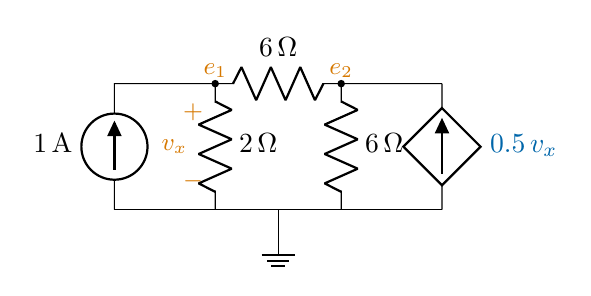
\begin{tikzpicture}[scale=0.8]
  \exD
\end{tikzpicture}
\end{minipage}\hfill
\begin{minipage}[c]{0.55\linewidth}
\textbf{Question.} Find $\e{1}$ and $\e{2}$. Treat the dependent source as a current source
$\Icol{0.5\,v_x}$; write its control $\Vcol{v_x}$ with node voltages:
\begin{alignat*}{2}
  &\text{node 1:}\ \ & -1 + \frac{\e{1}}{2} + \frac{\e{1} - \e{2}}{6} &= 0\\
  &\text{node 2:}\ \ & \frac{\e{2} - \e{1}}{6} + \frac{\e{2}}{6} - \Icol{0.5\,v_x} &= 0
\end{alignat*}
First plug $\Vcol{v_x} = \e{1}$ into node 2: $-\frac23\,\e{1} + \frac13\,\e{2} = 0$.
Then the matrix:
\[
  \begin{bmatrix} \frac23 & -\frac16\\[2pt] -\frac23 & \frac13 \end{bmatrix}
  \begin{bmatrix} \e{1}\\[2pt] \e{2} \end{bmatrix}
  = \begin{bmatrix} 1\\[2pt] 0 \end{bmatrix},
  \quad \e{1} = 3\V, \ \e{2} = 6\V.
\]
\end{minipage}
\end{examplebox}

\begin{examplebox}[Example 11.5 --- a dependent voltage source]
\begin{minipage}[c]{0.42\linewidth}
\centering
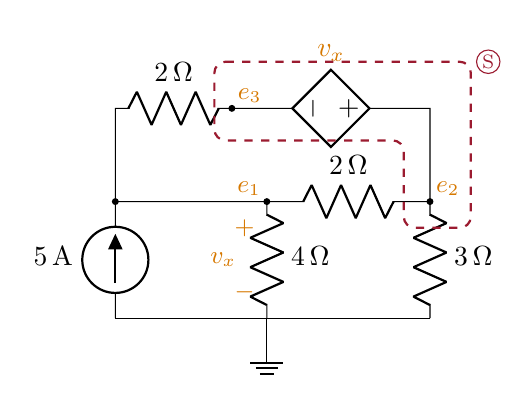
\begin{tikzpicture}[scale=0.74]
  \exC{1}
\end{tikzpicture}
\end{minipage}\hfill
\begin{minipage}[c]{0.55\linewidth}
\textbf{Question.} Find the power absorbed by the $3\ohm$ resistor.

The source $\Vcol{v_x}$ is between nodes 3 and 2, and neither is the ground. So use a
supernode \nd{S} around nodes 2 and 3. The unknowns are $\e{1}$, $\e{2}$, $\e{3}$.
\begin{alignat*}{2}
  &\text{(1) node 1:}\ \ & -5 + \frac{\e{1} - \e{3}}{2} + \frac{\e{1}}{4} + \frac{\e{1} - \e{2}}{2} &= 0\\
  &\text{(2) \nd{S}:}\ \ & \frac{\e{3} - \e{1}}{2} + \frac{\e{2} - \e{1}}{2} + \frac{\e{2}}{3} &= 0
\end{alignat*}
\end{minipage}
\end{examplebox}

\textbf{Constraint.} The source gives $\e{2} - \e{3} = \Vcol{v_x}$, and its control
$\Vcol{v_x}$ is the voltage of the $4\ohm$, so $\Vcol{v_x} = \e{1}$:
\[
  \e{2} - \e{3} = \e{1} . \qquad (3)
\]

\textbf{Solving Example 11.5.} Collect the terms of (1), (2) and (3), written as
$\e{1} - \e{2} + \e{3} = 0$:
\[
  \begin{bmatrix}
    \frac54 & -\frac12 & -\frac12\\[2pt]
    -1 & \frac56 & \frac12\\[2pt]
    1 & -1 & 1
  \end{bmatrix}
  \begin{bmatrix} \e{1}\\[2pt] \e{2}\\[2pt] \e{3} \end{bmatrix}
  = \begin{bmatrix} 5\\[2pt] 0\\[2pt] 0 \end{bmatrix}
  \quad\Rightarrow\quad \e{1} = 8\V, \ \e{2} = 9\V, \ \e{3} = 1\V .
\]
The $3\ohm$ is between node 2 and the ground, so
$\Pcol{P_{3\Omega}} = \e{2}^{\,2}/3 = 9^2/3 = \Pcol{27\W}$.

\begin{definitionbox}{Remark: a dependent voltage source to the ground}
If a dependent voltage source is between node $k$ and the ground, do not write KCL at node $k$:
its current is not known. Write its constraint instead.
\end{definitionbox}

%==============================================================
\section{Choosing a different ground}

Moving the ground shifts all node voltages by the same amount; branch quantities do not change.

\begin{examplebox}[Example 11.6 --- one circuit, two grounds]
\begin{minipage}[t]{0.48\linewidth}
\centering
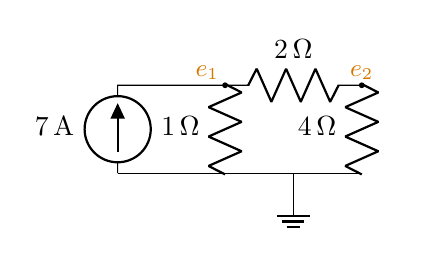
\begin{tikzpicture}[scale=0.62]
  \exG{3}{1}
\end{tikzpicture}\\
{\small ground at node 3}
\begin{align*}
  &\text{node 1:}\ \ -7 + \frac{\e{1}}{1} + \frac{\e{1} - \e{2}}{2} = 0\\
  &\text{node 2:}\ \ \frac{\e{2} - \e{1}}{2} + \frac{\e{2}}{4} = 0
\end{align*}
\[
  \begin{bmatrix} \frac32 & -\frac12\\[2pt] -\frac12 & \frac34 \end{bmatrix}
  \begin{bmatrix} \e{1}\\[2pt] \e{2} \end{bmatrix}
  = \begin{bmatrix} 7\\[2pt] 0 \end{bmatrix}
  \ \Rightarrow\ \begin{array}{l} \e{1} = 6\V\\ \e{2} = 4\V \end{array}
\]
\end{minipage}\hfill
\begin{minipage}[t]{0.48\linewidth}
\centering
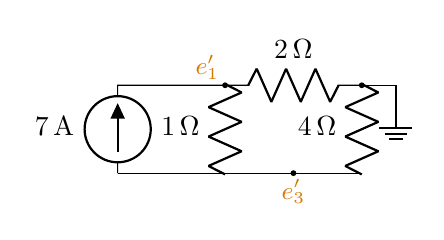
\begin{tikzpicture}[scale=0.62]
  \exG{2}{1}
\end{tikzpicture}\\
{\small ground at node 2}
\begin{align*}
  &\text{node 1:}\ \ -7 + \frac{\ep{1} - \ep{3}}{1} + \frac{\ep{1}}{2} = 0\\
  &\text{node 3:}\ \ 7 + \frac{\ep{3} - \ep{1}}{1} + \frac{\ep{3}}{4} = 0
\end{align*}
\[
  \begin{bmatrix} \frac32 & -1\\[2pt] -1 & \frac54 \end{bmatrix}
  \begin{bmatrix} \ep{1}\\[2pt] \ep{3} \end{bmatrix}
  = \begin{bmatrix} 7\\[2pt] -7 \end{bmatrix}
  \ \Rightarrow\ \begin{array}{l} \ep{1} = 2\V\\ \ep{3} = -4\V \end{array}
\]
\end{minipage}

\smallskip
\textbf{What changes?} $Y_n$ and the node voltages change: every node voltage shifts by
$-4\V$. The branch voltages do not: $\Vcol{v_{1\Omega}} = 6\V$, $\Vcol{v_{2\Omega}} = 2\V$,
$\Vcol{v_{4\Omega}} = 4\V$ in both. So the currents do not change either.
\end{examplebox}

\textbf{Tip.} Put the ground at one end of a voltage source: then its other node voltage is
known, or a supernode is avoided.

%==============================================================
\section*{Summary}

\begin{center}
\small
\renewcommand{\arraystretch}{1.15}
\begin{tabular}{@{}>{\raggedright}p{5.4cm} >{\raggedright\arraybackslash}p{10.3cm}@{}}
\toprule
\textbf{In the circuit} & \textbf{What to do}\\
\midrule
resistors and current sources & KCL at every non-ground node: $Y_n\Vcol{\mathbf{e}} =
  \Icol{\mathbf{i}_n}$, from three simple rules; $Y_n = A_R G A_R^T$ is symmetric\\
a voltage source, ground to node $k$ & $\e{k} = \Vcol{v_s}$ is known; no KCL at node $k$\\
a voltage source between nodes & Method I: its current as an unknown, plus the
  constraint;\newline Method II: KCL at the supernode, plus the constraint\\
a dependent source & write its control variable with node voltages: a constraint equation\\
the choice of ground & any node; the branch voltages and currents do not change\\
\bottomrule
\end{tabular}
\end{center}
After the node voltages are found: $\Vcol{\mathbf{v}} = A^T\Vcol{\mathbf{e}}$, then the
branch currents from the element laws.

\end{document}
